\documentclass[a4paper, 11pt]{article}%тип документа
\usepackage{siunitx}
%отступы
\usepackage[left=2cm,right=2cm,top=2cm,bottom=3cm,bindingoffset=0cm]{geometry}
\usepackage[pdftex]{lscape}
%Русский язык
\usepackage[T2A]{fontenc} %кодировка
\usepackage[utf8]{inputenc} %кодировка исходного кода
\usepackage[english,russian]{babel} %локализация и переносы

%Вставка картинок
\usepackage{wrapfig}
\usepackage{graphicx}
\graphicspath{{Images/}}
\DeclareGraphicsExtensions{.pdf,.png,.jpg}

%Математика
\usepackage{amsmath, amsfonts, amssymb, amsthm, mathtools}

\usepackage{amssymb}

%Заголовокhttps://www.overleaf.com/project/6507f5a4176b25bf05722230
\author{Акимов М.И., Кондратюк Н.А. \\ Б06-206}

\title{Отчёт о выполнении лабораторной работы  \\ \textbf{Кинетика обесцвечивания красителей.}}
\date{\\24 апреля 2024 года}
\begin{document}

\maketitle
\section{Цель работы.}
    \par Исследовать кинетику реакции обесцвечивания красителя на примере фенолфталеина и NaOH, на основе полученных измерений определить порядок и константу скорости реакции. Исследовать влияние ионной силы раствора на скорость реакции.
\section{Задачи работы.}
    \begin{itemize}
        \item В начале работы необходимо снять спектр поглощения раствора фенолфталеина с целью определения пика поглощения для дальнейших измерений.
        \item Приготовить ряд растворов разной концентрации щёлочи и с помощью спектрофотометра зарегистрировать обесцвечивание при протекании реакции с фенолфталеином.
        \item Воспользоваться методом избыточных концентраций и с помощью линеаризации зависимостей расчитать эффективные константы скорости реакции. Исследовать поведение кинетической кривой, предположить частный порядок реакции по фенолфталеину.
        \item Из зависимости эффективных констант скоростей от концентрации NaOH в растворе расчитать истинную константу скорости и частный порядок реакции по щёлочи.
        \item Приготовить ряд растворов одинаковых по концентрации щёлочи, но разных по ионной силе, и с помощью спектрофотометра зарегистрировать обесцвечивание при протекании реакции с фенолфталеином.
        \item На основе полученных данных построить кривые, отвечающие растворам с известной ионной силой; провести их линеаризацию, определив таким образом константы скоростей в каждом опыте; отметить характер зависимости констант от ионной силы в двух приближениях теории Дебая-Хюккеля; сделать вывод о соответствии полученных данных теоретическим зависимостям.
        
    \end{itemize}

\section{Теоретическое введение.}
\subsection{Кинетика реакции обесцвечивания фенолфталеина в сильно щелочной среде.}\;
\par Фенолфталеин - трифенилметановый краситель, кислотно-основный индикатор. При $pH \approx 8$ и меньше молекула фенолфталеина находится в протонированной форме. При $pH$ в диапазоне от 8 до 10 протоны отщепляются основанием, что приводит к образованию иона с характерной розовой окраской. Если $pH$ становится больше 10, то розовая окраска медленно исчезает с образованием бесцветного иона по реакции:
$$P^{2-}_{aq} + OH^-_{aq} \leftrightarrows POH^{3-}_{aq}$$
\par Кинетическое уравнение этой реакции имеет следующий вид:
\begin{equation*}
    w = k_2 [P^{2-}]^m[OH^-]^n
    \eqno(1)
\end{equation*}
\par Лабораторные эксперименты в работе будут проводиться при концентрациях щёлочи, много раз превышающих концентрацию фенолфталеина. Следовательно, в течение реакции концентрацию гидроксида натрия можно считать постоянной:
$$w = k_1[P^{2-}]^m$$
\begin{equation*}
    k_1 = k_2[OH^-]^n
    \eqno(2)
\end{equation*}
\par Таким образом, измеряя скорость реакции при нескольких разных концентрациях щёлочи, можно будет определить частный порядок реакции по $NaOH$ и величину константы скорости $k_2$.
\subsection{Использование спектрофотометрических методов.}\;
\par Данные в работе будут определяться на основе спектрофотометрических измерений, позволяющих зафиксировать изменение концентрации окрашенной формы фенолфталеина в растворе. По закону Бугера-Ламберта-Бера:
\begin{equation*}
    D = \varepsilon_{\lambda} C l
    \eqno(3)
\end{equation*}
\par Для реакции первого или псевдопервого порядка константа скорости может быть выражена, как:
\begin{equation*}
    k_1 = \frac{1}{t}ln\frac{C_0}{C(t)}= \frac{1}{t}ln\frac{D_0}{D(t)}
    \eqno(4)
\end{equation*}
\subsection{Влияние среды на скорость ионных реакций.}\;
\par В теории переходного состояния скорость химической реакции определяется выражением:
\begin{equation*}
    w = \frac{k_bT}{h} C^{\#}
    \eqno(5)
\end{equation*}
\par В данной теории постулируется существование равновесия между исходными реагентами и активированным комплексом. В частности, для бимолекулярной реакции с участием заряженных частиц A и B в растворе можно получить концентрацию активированного комплекса, используя следующите выражения:
$$K^\#_a = \frac{C^\#}{C_AC_B} \cdot \frac{\gamma^\#}{\gamma_A\gamma_B}$$

\begin{equation*}
    C^\# = K^\#_a\frac{\gamma_A\gamma_B}{\gamma^\#}\frac{1}{C_AC_B}
    \eqno(6)
\end{equation*}
\par Коэффициенты по теории Дебая-Хюккеля определяются:
\begin{equation*}
    -lg(\gamma) = 1,823 \cdot 10^6 (\varepsilon T)^{-3/2}Z^2\sqrt{I}
    \eqno(7)
\end{equation*}
\par Преобразуя комбинацию коэффициентов активности в этом выражении, получим:
\begin{equation*}
    lg\frac{k}{k_0} = 2AZ_AZ_B\sqrt{I}
    \eqno(8)
\end{equation*}
\section{Ход работы.}
\subsection{Исследование зависимости кинетики реакции от концентрации NaOH}
    \par В начале работы был снят спектр поглощения раствора фенолфталеина при небольшом добавлении щёлочи в диапозоне 200 - 700 нм (Рис. 1). Был определён максимум поглощения 553 нм, при котором проводились все дальнейшие измерения.
    \begin{figure}[h!]
    	\centering{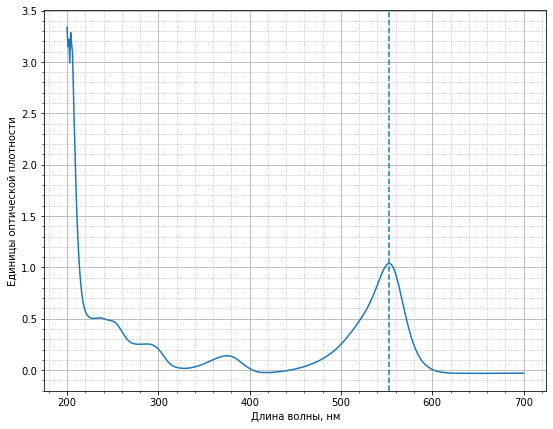
\includegraphics [scale=0.5]{Images/фенолфталеин.png}}
            \caption{Спектр поглощения раствора фенолфталеина в слабощелочной среде.}
    \end{figure}
    \par Для исследования зависимости кинетики реакции обесцвечивания от концентрации щёлочи были приготоволены 8 растворов NaOH разной концетрации (Таблица 1). Для поддержания одинаковой ионной силы в каждом эксперименте использовался 0,3 М раствор NaCl.
    \begin{table}
        \centering
        \begin{tabular}{|l|l|l|l|l|l|}
        \hline
            Раствор & $C_{NaOH}$, М & $V_{NaOH}$, мл & $V_{NaCl}$, мл & $k_1 \cdot 10^{-3}$, 1/c & $k'_1 \cdot 10^{-3}$, 1/c\\ \hline
            C 1 & 0,05 & 0,5 & 2,5 & 1,60 & 2,67  \\ \hline
            C 2 & 0,10 & 1,0 & 2,0 & 3,28 & 4,38  \\ \hline
            C 3 & 0,13 & 1,3 & 1,7 & 4,36 & 5,70  \\ \hline
            C 4 & 0,16 & 1,6 & 1,4 & 5,20 & 6,71  \\ \hline
            C 5 & 0,19 & 1,9 & 1,1 & 6,36 &  7,91  \\ \hline
            C 6 & 0,22 & 2,2 & 0,8 & 7,36 & 7,96  \\ \hline
            C 7 & 0,25 & 2,5 & 0,5 & 8,56 & 10,07  \\ \hline
            C 8 & 0,30 & 3,0 & 0,0 & 10,48 & 12,37  \\ \hline
        \end{tabular}
        \caption{Параметры растворов и результаты измерений при разных концентрациях NaOH.}
    \end{table}
    \par Изначально мы предполагали найти эффективные константы скорости реакции $k_{1} = k_{2} \cdot [OH^{-}]^{n}$ с помощью линеаризации в полулогарифмических координатах $ln(\frac{D(t)}{D_0})(t)$. Однако на графике (Рис. 2) кинетической кривой в этих координатах видно, что, начиная с какого-то момента времени, значения выходят на плато, что говорит об идущей обратной реакции. Поэтому для более точного результата дополнительно произведём линеаризацию в координатах $ - \frac {dD}{dt} (D)$ (Рис. 3). Из уравнения прямой находим $k_{1}$ и $k'_{1}$ для каждой концентрации (Таблица 1).
    \begin{figure}[!htb]
        \minipage{0.47\textwidth}
            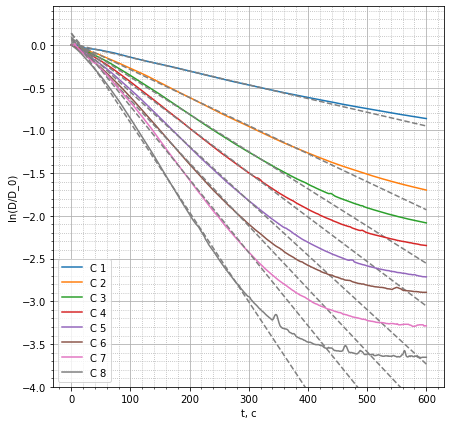
\includegraphics[width=\linewidth]{Images/ln(DкD0)(t).png}
            \caption{График зависимости $ln(\frac{D(t)}{D_0})(t)$ при разных концентрациях NaOH.}
        \endminipage\hfill
        \minipage{0.47\textwidth}
            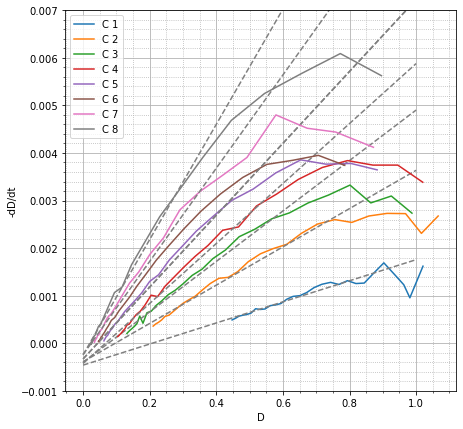
\includegraphics[width=\linewidth]{Images/dDкdt(D).png}
            \caption{График зависимости $ - \frac {dD}{dt} (D)$ при разных концентрациях NaOH.}
        \endminipage
    \end{figure}
    \par Для определения частного порядка реакции по NaOH и константы скорости реакции $k_{2}$ воспользуемся двойными логарифмическими координатами, а именно построим зависимость $\ln{k_1}$ от $\ln{C_{NaOH}}$, из угла наклона определим порядок реакции p, а из свободного члена - $k_{2}$ (Рис.). 
    \begin{figure}[!htb]
        \minipage{0.48\textwidth}
            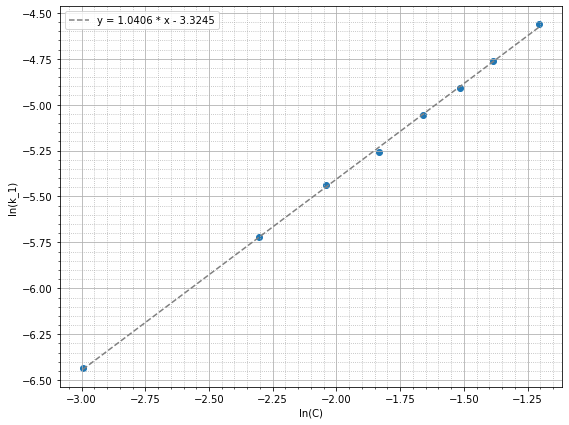
\includegraphics[width=\linewidth]{Images/norm_linear.png}
            \caption{График зависимости $\ln{k_1} (\ln{C_{NaOH}})$ для линеаризации через $ln(\frac{D(t)}{D_0})$.}
        \endminipage\hfill
        \minipage{0.48\textwidth}
            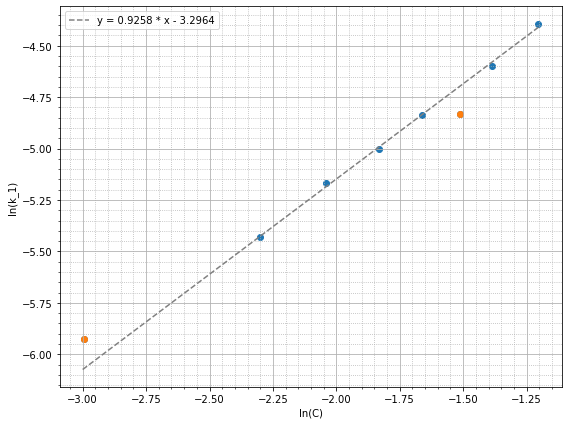
\includegraphics[width=\linewidth]{Images/ln(k_1)(lnC).png}
            \caption{График зависимости $\ln{k'_1} (\ln{C_{NaOH}})$ для линеаризации через производные.}
        \endminipage
    \end{figure}
    
    \par Из аппроксимации получаем частный порядок реакции по гидроксилам:
    $$p = 1,04 \approx 1$$
    $$p' = 0,93 \approx 1$$ 
    \par И константу скорости реакции:
    $$k_2 = e^{-3,325} \approx 0.036 \ \mathrm{M}^{-1} \cdot c^{-1}$$
    $$k'_2 = e^{-3,296} \approx 0.037 \ \mathrm{M}^{-1} \cdot c^{-1}$$
\newpage
\subsection{Исследование зависимости скорости реакции от ионной силы раствора.} \;
\par В данной части работы будем изменять ионную силу растовора с исследуемым красителем и отмечать, как при этом будет изменяться константа скорости реакции обесцвечивания фенолфталеина. 
\par Исследуемые растворы будут обладать следующими количественными параметрами (Таблица 2).
\begin{table}[h!]
\centering
\caption{Параметры растворов.}
\begin{tabular}{|l|l|l|l|}
\hline
$C_{NaOH}, \; \text{М}$ & $I, \; \text{М}$ & $V_{NaOH}, \; \text{мл}$ & $V_{NaCl}, \; \text{мл}$ \\ \hline
0,1 & 0,1 & 1 & 0,000 \\ \hline
0,1 & 0,4 & 1 & 0,375 \\ \hline
0,1 & 0,7 & 1 & 0,750 \\ \hline
0,1 & 1,0 & 1 & 1,125 \\ \hline
0,1 & 1,3 & 1 & 1,500 \\ \hline
0,1 & 1,5 & 1 & 1,750 \\ \hline
0,1 & 1,7 & 1 & 2,000 \\ \hline
\end{tabular}
\end{table}

\par Построим графики зависимости оптической плотности (а вернее, отношения величины оптической плотности в данный момент времени к величене оптической плотности в начальной) от времени в обычных и полулогарифмических координатах (Рис. 6 и 7).

            \begin{figure}[!htb]
                \minipage{0.45\textwidth}
                 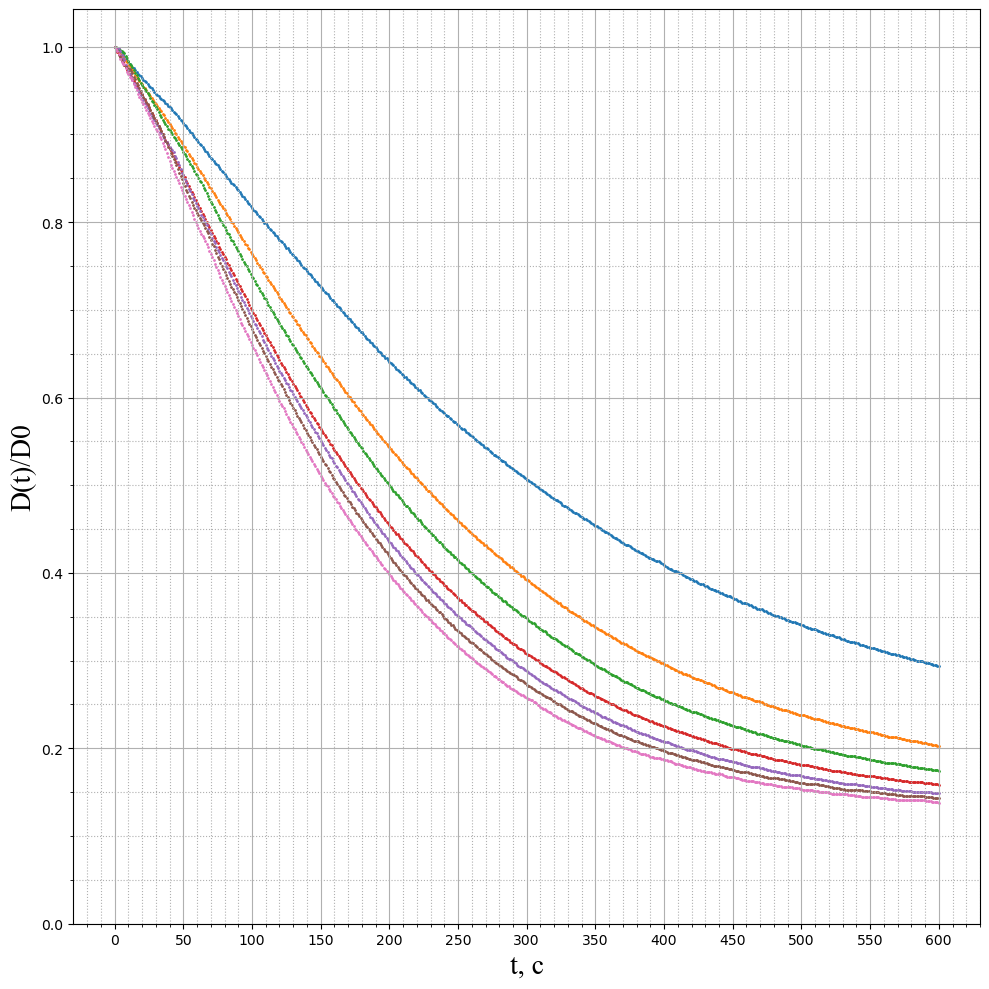
\includegraphics[width=\linewidth]{Images/Кинетика1.png}
                 \caption{График зависимости $\frac{D(t)}{D_0}(t)$.}
                  \endminipage\hfill
                \minipage{0.45\textwidth}
                 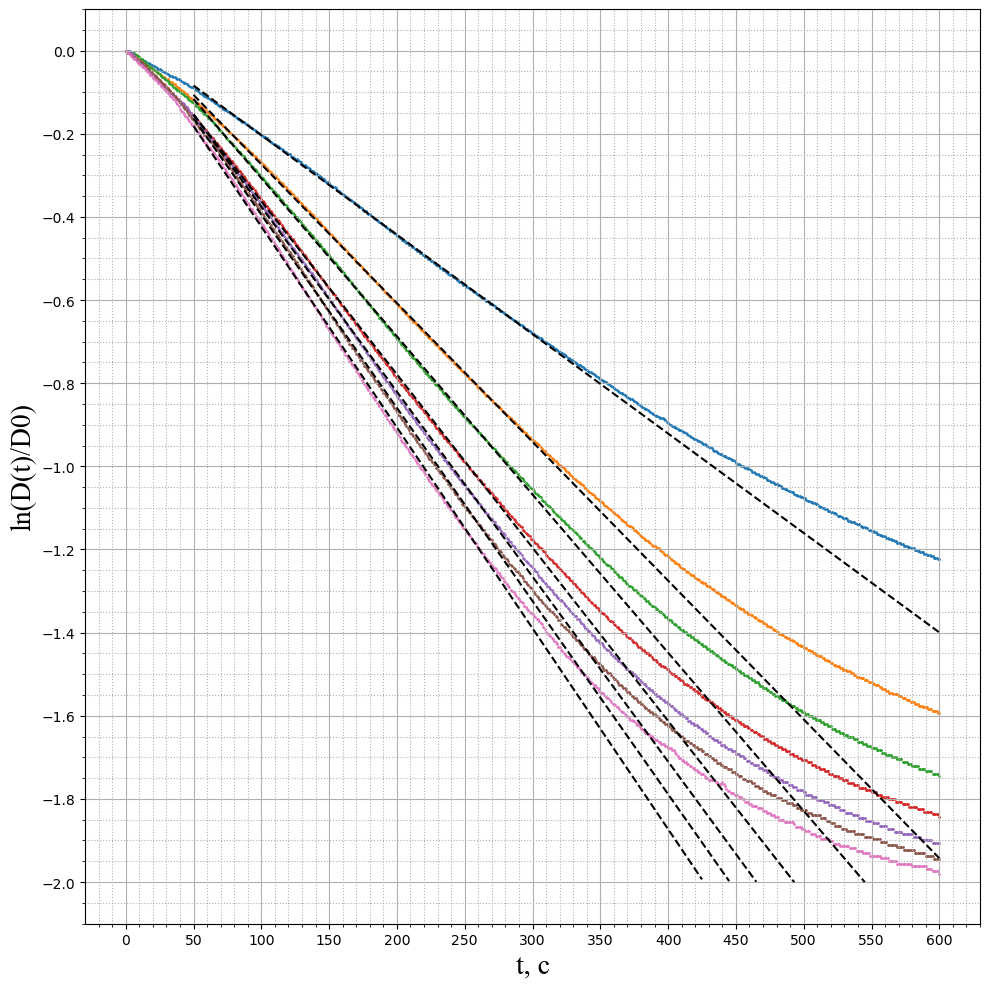
\includegraphics[width=\linewidth]{Images/Кинетика2.png}
                 \caption{График зависимости $ln(\frac{D(t)}{D_0})(t)$.}
                  \endminipage
              \end{figure}
\par На основе теоретических соображений зависимость, представленная на Рис. 6 должна быть спрямляема в координатах на Рис. 7. Как видно на Рис. 7, спрямляемость выполняется только на определённом участке кривой. Поэтому для большей точности проведём спрямление функций $\frac{d D}{d t} (D)$ (Рис. 8).
 \begin{figure}[h!]
	\centering{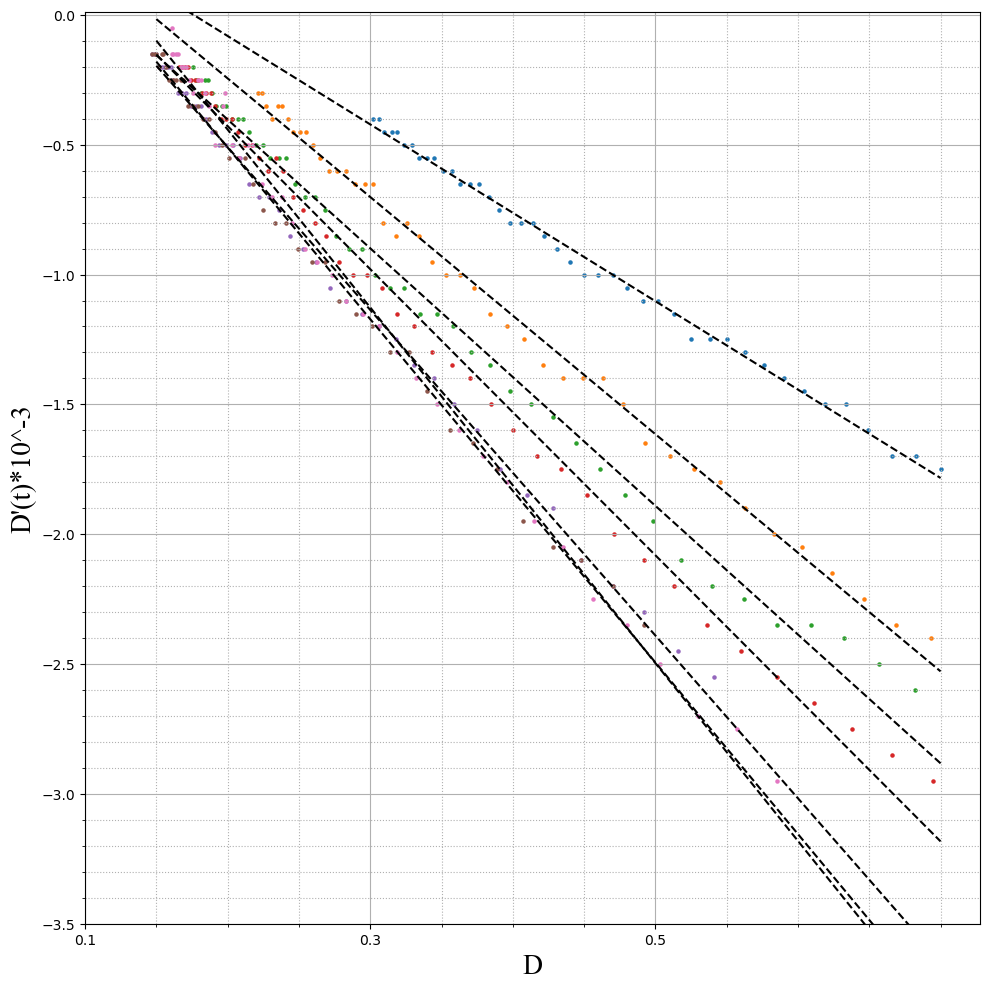
\includegraphics [scale=0.3]{Images/Кинетика3.png}}
        \caption{График зависимости $\frac{d D}{d t} (D)$.}
    \end{figure}
\par Таким образом, получим коэффициенты наклона зависимостей и привидём их в Таблице 3.
\begin{table}[h!]
\centering
\caption{Коэффициенты наклона.}
\begin{tabular}{|l|l|l|}
\hline
$I, \; \text{М}$  & $k, \;  10^{-3} \frac{1}{\text{с}}$ & $k', \;  10^{-3}\frac{1}{\text{с}}$ \\ \hline
0,1 & 2,39 & 3,40 \\ \hline
0,4 & 3,34 & 4,57 \\ \hline
0,7 & 3,80 & 4,96 \\ \hline
1,0 & 4,17 & 5,51 \\ \hline
1,3 & 4,45 & 6,27 \\ \hline
1,5 & 4,65 & 6,61 \\ \hline
1,7 & 4,83 & 6,85 \\ \hline
\end{tabular}
\end{table}
\par Полученные данные соотнесём с корнем из ионной силой, произведя пересчёт теоретического коэффициента $A$, исходя из используемой температуры:
$$A = \frac{1,88 \cdot 10^6}{(\varepsilon T)^{3/2}} = 0,4976 \; \frac{1}{\sqrt{\text{М}}}$$
\par Таким образом, вычислим по углу наклона графика $lg(k)(\sqrt{I})$. 
Для этого будем использовать первое и второе приближения Теории Дебая - Хюккеля (Рис. 9 и Рис. 10). Полученные значения приведём в Таблице 4.
\begin{figure}[!htb]
                \minipage{0.45\textwidth}
                 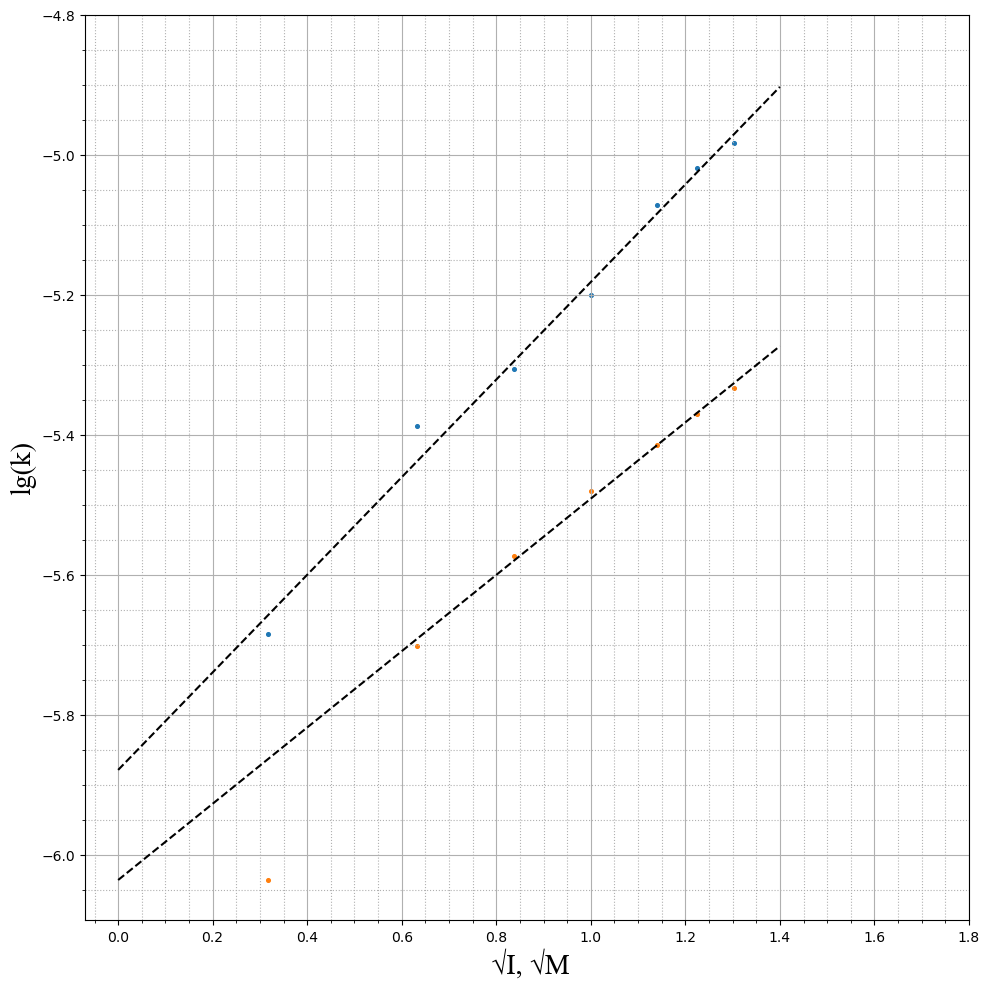
\includegraphics[width=\linewidth]{Images/Кинетика4.png}
                 \caption{Первое приближение Дебая - Хюккеля.}
                  \endminipage\hfill
                \minipage{0.45\textwidth}
                 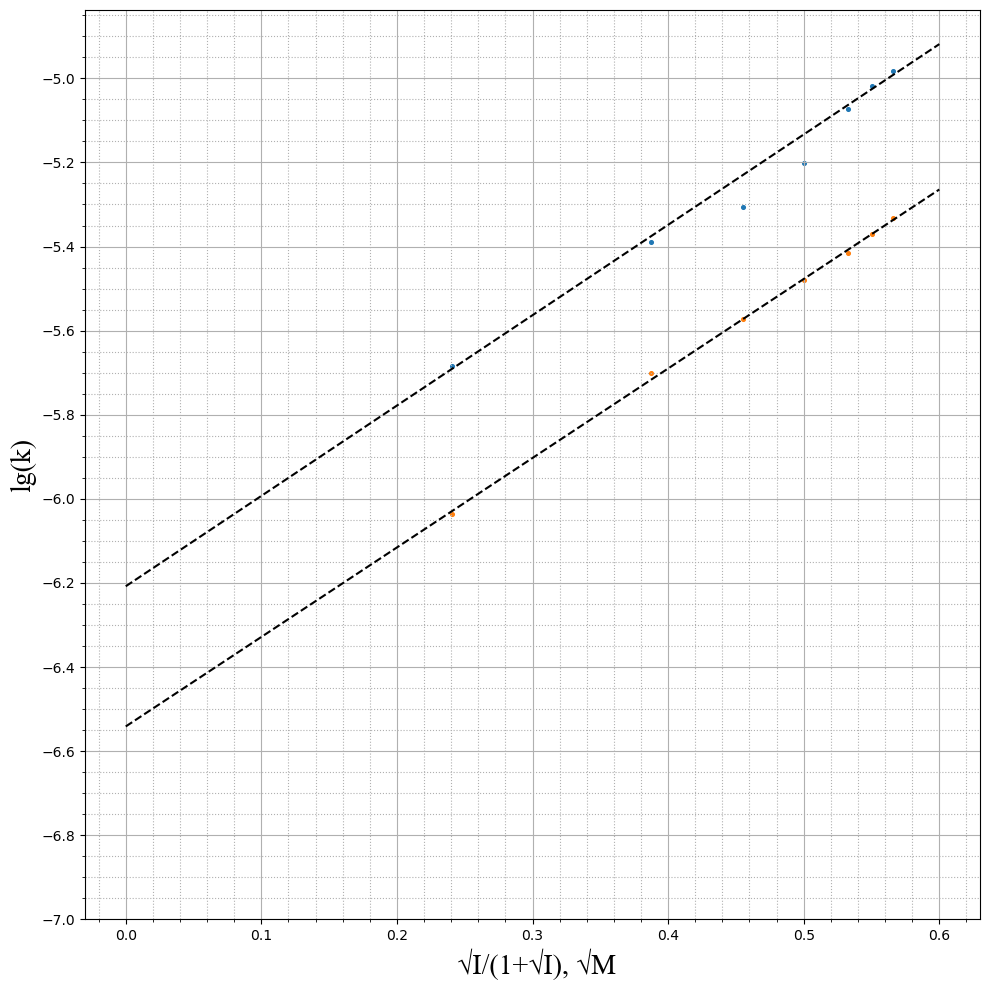
\includegraphics[width=\linewidth]{Images/Кинетика5.png}
                 \caption{Второе приближение Дебая - Хюккеля.}
                  \endminipage
              \end{figure}
\begin{table}[h!]
\centering
\caption{Произведение зарядов из угла наклона соответствующих графиков.}
\begin{tabular}{|l|l|l|}
\hline
 & $Z_AZ_B$ & $Z_A'Z_B'$ \\ \hline
Первое приближение & 0,69 & 0,70 \\ \hline
Второе приближение & 2,14 & 2,13 \\ \hline
\end{tabular}
\end{table}
\par В итоге, приходим к выводу, что найденные нами по второму приближению в обоих случаях (в двух линеаризациях) значения являются близкими к реальному $Z_AZ_B = 2$. 
\newpage
\section{Выводы.}
    \begin{itemize}
        \item При исследовании кинетики реакции обесвечивания фенолфталеина был выявлен весомый для кинетической кривой вклад обратной реакции.
        \item С помощью метода избыточных концентраций был определён частный порядок реакции по NaOH $p \approx 1$.
        \item Применяя разные способы линеаризации, была установлена истинная константа скорости реакции обесцвечивания красителя $k_{2} \approx 0.036 \ \mathrm{M}^{-1} \cdot c^{-1}$.
        \item Установили, что при увеличении ионной силы раствора константа скорости тоже увеличивалась, что соответствует одноимённо заряженным ионам.
        \item Был произведён пересчёт коэффициента A, так как реакция проводилась при включённом на 39 $C^{\circ}$ термостате.
        \item На основе вычисления углов наклона зависимостей $lg(k)(\sqrt{I})$ и $lg(k)(\frac{\sqrt{I}}{1+\sqrt{I}})$ получим значения произведения зарядов ионов, которые участвуют в реакции. Отметим, что величина произведения, посчитанная на основе второго приближения Дебая-Хюккеля, лучше совпадает с таковой теоретической, а именно $Z_AZ_B = 2$.
    \end{itemize}
\end{document}
